\section{Zielsetzung}
Laser (\textbf{l}ight \textbf{a}mplification by \textbf{s}timulated \textbf{e}mission of \textbf{r}adiation) sind in der experimentellen Physik von zentraler Bedeutung
und werden u.a. zur Untersuchung atomarer Strukturen genutzt. Sie bieten eine leistungsstarke Quelle für kohärentes Licht und sind 
oft auf bestimmte Wellenlängen einstellbar. In diesem Versuch wird die Funktionsweise eines Diodenlasers, die Justierung des Lasers
und dessen Bedienung im Experiment am Beispiel des Absorptionsspektrums von Rubidium erprobt.


\section{Theorie}
\label{sec:Theorie}

\subsection{Zustandssysteme und Besetzungsinversion}
\label{subsec:Theorie_Zustandssysteme}
Das Funktionsprinzip eines Lasers beruht auf der quantenmechanischen Beschreibung von Zustandssystemen. Demnach lassen sich Systeme von Teilchen (z.B. Elektronen oder Atome)
durch ein Zustandssystem beschreiben, bei dem jedem möglichen Zustand eine Energie zugeordnet wird. Damit ein Teilchen in einen energetisch höheren Zustand gelangen kann,
muss es genau die Energiedifferenz zwischen den beiden Zuständen überwinden. Dies ist über die Absorption eines Photons möglich, dessen Frequenz $\nu$ genau zur nötigen 
Energie $E = \symup{h}\nu$ korrespondiert. Ebenso wird bei einem Übergang in ein niedrigeres Niveau Energie frei, die in Form eines Photons emittiert wird. Ein solcher 
Übergang kann spontan auftreten (spontane Emission) oder durch ein Photon gleicher Frequenz angeregt werden (stimulierte/induzierte Emission). Bei stimulierter Emission
stimmt das emittierte Photon in Frequenz, Phasenlage und Polarisation mit dem anregenden Photon überein, weshalb dieser Vorgang zur Erzeugung von kohärentem Licht in einem 
Laser genutzt wird. Dazu müssen jedoch die energetisch höheren Zustände stets stärker besetzt sein, als energetisch Niedrige, damit die stimulierte Emission überwiegen kann. 
Dies wird \textit{Besetzungsinversion} genannt. Bei einem Zwei-Zustandssystem mit Energien $E_1 < E_2$ ist dies nicht möglich, da die Wahrscheinlichkeiten der Übergänge
$E_1 \to E_2$ und $E_2 \to E_1$ gleich sind und sich somit maximal eine Gleichverteilung auf die Zustände einstellen könnte. Gibt es jedoch einen weiteren Zustand zwischen
den Energieniveaus $E_1$ und $E_2$ kann Besetzungsinversion erreicht werden. Das Anregungsschema eines 4-Niveau Systems ist in \autoref{fig:4Niveau} abgebildet.
\begin{figure}
    \centering
    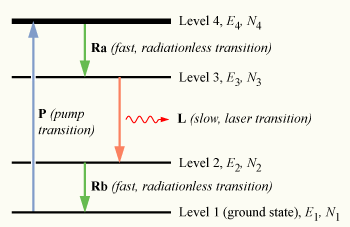
\includegraphics[scale=0.58]{content/pics/Population-inversion-4level.png}
    \caption{Anregungsschema eines 4-Niveau-Lasers. Zwischen Niveau 3 und 2 wird ein Photon durch stimulierte Emission ausgesendet. \cite{wikipedia_population_inversion}}
    \label{fig:4Niveau}
\end{figure}
Die Elektronen werden in das höchste Energieniveau \dq gepumpt\dq{} und fallen schnell in das kurz darunter liegende Niveau 3 ab. Dies geschieht mitunter sogar strahlungsfrei.
Zwischen den Niveaus 3 und 2 findet stimulierte Emission statt. Anschließend fällt das Elektron schnell und strahlungsfrei aus dem zweiten Zustand - welcher kurz über dem Ersten
liegt - in den Grundzustand zurück, aus dem es wieder in den vierten Zustand gepumpt werden kann. Durch diese Anordnung liegt immer Besetzungsinversion vor.

\subsection{Funktionsweise von Halbleiterdioden}
Eine Halbleiterdiode besteht im wesentlichen aus einem p- und einem n-dotierten Halbleitermaterial. Eine \glqq Dotierung\grqq{} meint das Einbringen von Fremdatomen in ein
Grundmaterial. Negativ geladenen Atome bringen dabei zusätzliche Elektronen in das Material, welche sich frei bewegen können. Diese Art von Dotieratomen werden Elektronendonatoren
genannt. Positiv geladene Atome werden Elektronenakzeptoren bringen \dq Fehlstellen\dq{} - auch Löcher genannt - in das Material, die sich ebenfalls frei bewegen können 
und sich wie positive Elektronen verhalten. Bei n-Dotierung entsteht ein Donatorniveau knapp unter dem Leitungsband des Materials, bei p-Dotierung ein Akzeptorniveau knapp 
über dem Valenzband. Diese können schon durch geringfügige thermische Anregung (Raumtemperatur) besetzt werden, wodurch die Anzahl der freien Ladungsträger und somit auch die 
Leitfähigkeit steigt. 
Im Übergang einer p- zu einer n-dotierten Schicht bilden sich durch den Austausch von Löchern aus der p-dotierten Schicht und Elektronen aus der n-dotierten Schicht Bereiche 
positiver Ladung in der n-dotierten Schicht und negativer Ladung in der p-dotierten Schicht. Die dadurch bedingte Coulombkraft führt dazu, dass keine freien Ladungsträger 
im pn-Übergang verweilen könnnen und dieser somit wie ein Isolator fungiert. Dieser Bereich wird \textit{Verarmungszone} oder \textit{Sperrschicht} genannt.
Wird ein Strom an das Material angelagt, sodass die negativ dotierte Schicht mit dem negativen Pol der Stromquellen verbunden ist, wirkt die anliegende Spannung diesem 
Effekt entgegen, weshalb Strom zwischen den Schichten fließen kann. Elektronen rekombinieren dann mit Löchern im Valenzband der p-dotierten Schicht, wodurch ein Photon
emittiert wird, dessen Energie ungefähr der Bandlücke $E_G$ des Materials entspricht. Valenzband und Akzeptorniveau, sowie Donatorniveau und Leitungsband entsprechen 
den Energieniveaus des 4-Zustandssystems aus \autoref{subsec:Theorie_Zustandssysteme}, was bedeutet, dass Besetzungsinversion vorliegt. 
Die emittierten Photonen können ihrerseits wieder Emission weiterer Photonen gleicher Wellenlänge anregen.

\subsection{Aufbau eines Diodenlasers}
Das Herzstück eines Lasers ist der Diodenchip, in dem durch die oben beschriebenen Prozesse kohärentes Licht emittiert werden. Die gewünschte Wellenlänge der Photonen lässt sich 
über den Diodenstrom und die Diodentemperatur regulieren. Der Aufbau einer solchen Diode ist in \autoref{fig:LDChip} zu sehen. Die Grafik zeigt eine stehende Welle, die sich in 
der Diode bildet, da diese wie ein optischer Hohlraumresonator wirkt. Dies ist möglich, da die Front- und Rückseite der Diode (teilweise) reflektieren. 
In einer Diode der Länge $L$ aus einem Material mit Brechungsindex $n$ können Wellen der Wellenlänge $\lambda = \sfrac{2L}{k}  \;,k \in \mathbb{N}$ entstehen, die in der Frequenz 
eine Periodizität von 
\begin{equation}
    \label{eq:delta_nu}
    \Delta \nu = \frac{c}{2Ln}
\end{equation}  
vorweisen.

\begin{figure}
    \centering
    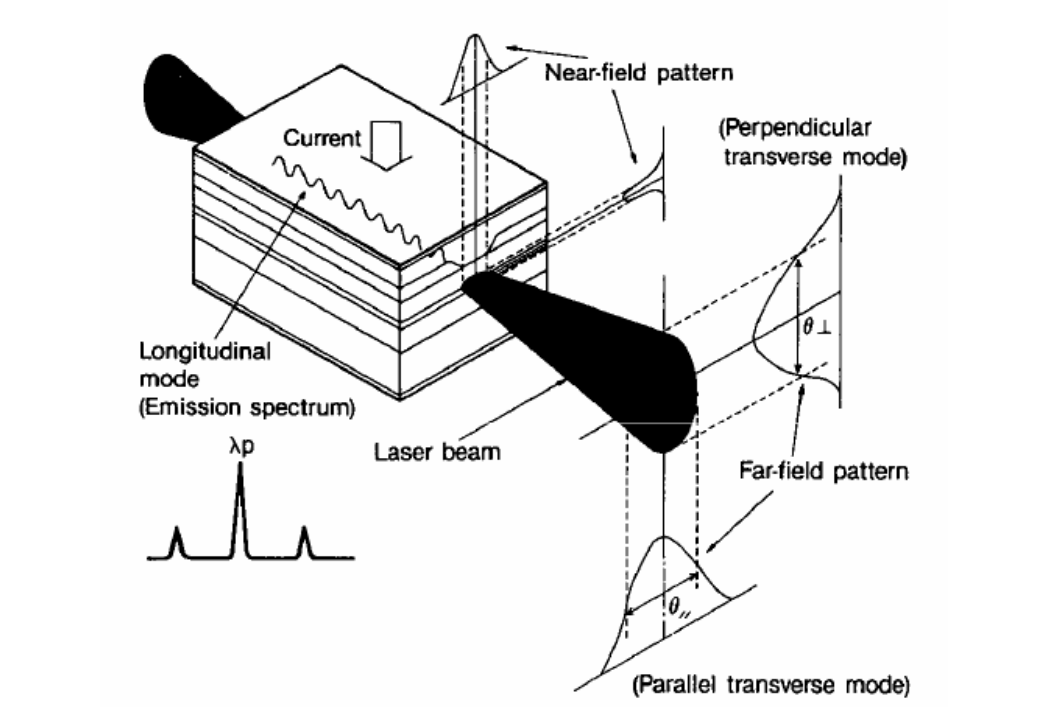
\includegraphics[scale=0.4]{content/pics/LDChip.png}
    \caption{Schematische Abbildung eines Laser-Diodenchips. Es sind einzelne Schichten der Diode und eine stehende Welle erkennbar. \cite{diode_laser_spectroscopy}}
    \label{fig:LDChip}
\end{figure}
